\chapter{Startup Vision: Launching Korpor}

% % Add a subtle decorative rule below the chapter title
% \begin{center}
% \begin{tikzpicture}
%   \draw[color=accent, line width=0.8pt, rounded corners=1pt] (0,0) -- (\textwidth*0.7,0);
% \end{tikzpicture}
% \end{center}
% \vspace{1.5em} % Add space after the rule

\section{Introduction}

This chapter outlines the prospective journey of transforming the Korpor project into an independent startup venture. It details the vision, the strategic arrangement with the sponsoring company, and includes key legal documents underpinning this transition.

\vspace{1cm} % Add some vertical space

\begin{tcolorbox}[
    enhanced,
    colback=background!95!white, % Slightly off-white background
    colframe=primary, % Primary color frame
    boxrule=1pt,
    arc=3mm, 
    outer arc=1mm,
    drop shadow={opacity=0.4, color=secondary}, % Add a subtle shadow
    title={\textbf{\color{white}The Entrepreneurial Leap}}, % White text on primary background
    fonttitle=\bfseries, 
    coltitle=primary, % Background for the title bar
    attach boxed title to top center={yshift=-2mm},
    boxed title style={colback=primary, arc=2mm} % Style the title box
]
\firstparagraph{T}he culmination of this project is not merely the delivery of a functional platform, but the foundation for \textbf{my future tech company, Korpor}. The sponsoring company has graciously agreed to provide the core application codebase, enabling the launch of this independent startup. Korpor will be dedicated to the continuous development and enhancement of this real estate investment platform.

This section will elaborate on the operational model for Korpor, focusing on its evolution into a Software-as-a-Service (SaaS) provider for the wider real estate industry, its market strategy, and its potential impact.

\vspace{1em} % Add space before QR code
\begin{center}
    
\includegraphics[width=0.25\textwidth]{images/korpor-qr.png} \\ % Include the QR code image
    \vspace{0.5em}
    \small\textit{Scan to visit the Korpor page.}
\end{center}
\vspace{0.5em} % Add space after QR code
\end{tcolorbox}

\section{Founding Documents}

\begin{tcolorbox}[
    enhanced,
    breakable, % Allow box to break across pages if needed
    colback=accent!25, % Darker accent background
    colframe=accent!70!black, % Slightly less dark accent frame
    boxrule=0.8pt,
    arc=1mm,
    title={\textbf{\color{white}Legal Framework}},
    fonttitle=\bfseries,
    coltitle=accent!50!primary % Richer title background
]
This section contains the formal documentation establishing the legal groundwork for the Korpor startup. The primary document included signifies the official handover of the application codebase developed during the initial project phase.


This agreement, originating from the project lead, confirms the transfer of the core technology to the new venture, Korpor, paving the way for its independent operation and future development as a SaaS provider.
\end{tcolorbox}

\vspace{1cm} % Add space after the box

\section{Path Forward}

\begin{tcolorbox}[
    enhanced,
    colback=primary!15, % More intense primary background
    colframe=primary!80!black, % Darker primary frame
    boxrule=0.8pt,
    arc=1mm,
    title={\textbf{\color{white}Strategic Roadmap}}, % White title text
    fonttitle=\bfseries,
    coltitle=primary % Solid primary title background
]
With the application codebase secured and the legal groundwork laid, the strategic path forward for \textbf{Korpor as my tech company} involves several key milestones:
\begin{itemize}[leftmargin=*, itemsep=0.5em]
    \item[\textcolor{primary}{\ding{226}}] \textbf{Secure Funding:} Actively pursue seed funding to support initial operations, team expansion, and marketing efforts.
    \item[\textcolor{primary}{\ding{226}}] \textbf{Build the Core Team:} Recruit talented individuals for key roles in development, marketing, sales, and operations.
    \item[\textcolor{primary}{\ding{226}}] \textbf{Develop SaaS Model:} Refine the platform architecture and features to support a scalable, multi-tenant Software-as-a-Service offering.
    \item[\textcolor{primary}{\ding{226}}] \textbf{Iterate and Enhance:} Continuously improve the platform based on user feedback and market analysis, focusing on delivering exceptional value to client companies.
    \item[\textcolor{primary}{\ding{226}}] \textbf{Market Penetration:} Implement a targeted marketing strategy to acquire initial real estate company clients and build brand presence.
\end{itemize}
The ultimate goal is to establish Korpor as a trusted and innovative SaaS provider, empowering other real estate businesses with advanced technology solutions. 
\end{tcolorbox} 


\begin{center}
% Uncomment and update this line when the final agreement PDF is ready
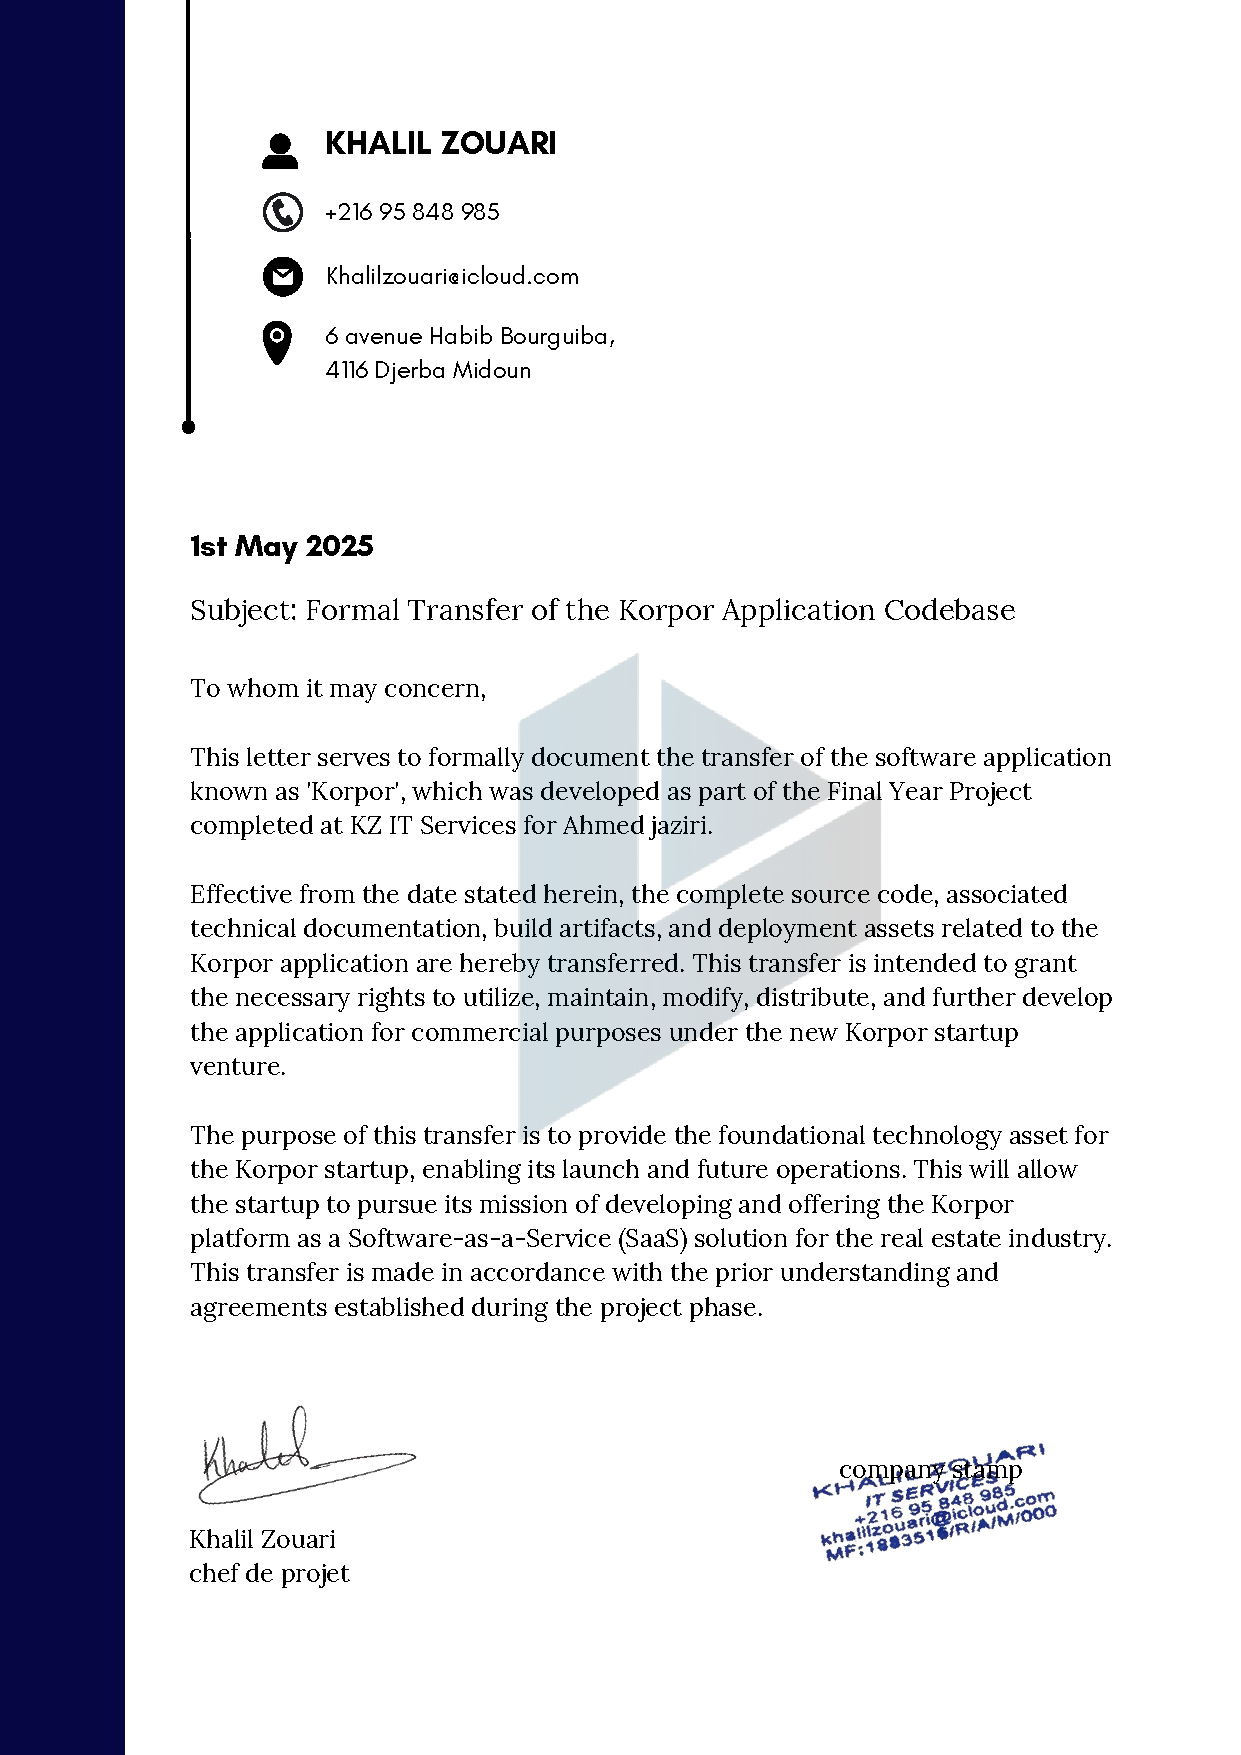
\includepdf[pages=-, pagecommand={\thispagestyle{fancy}}]{agreement.pdf} 
\end{center}
\newpage